\begin{figure}[htbp]
\centering
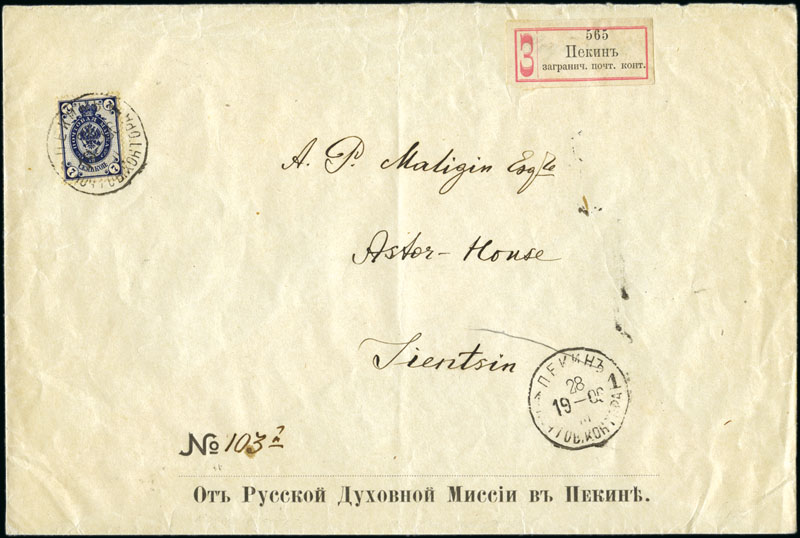
\includegraphics[width=.95\textwidth]{../russian-post-offices-in-china/10037.jpg}
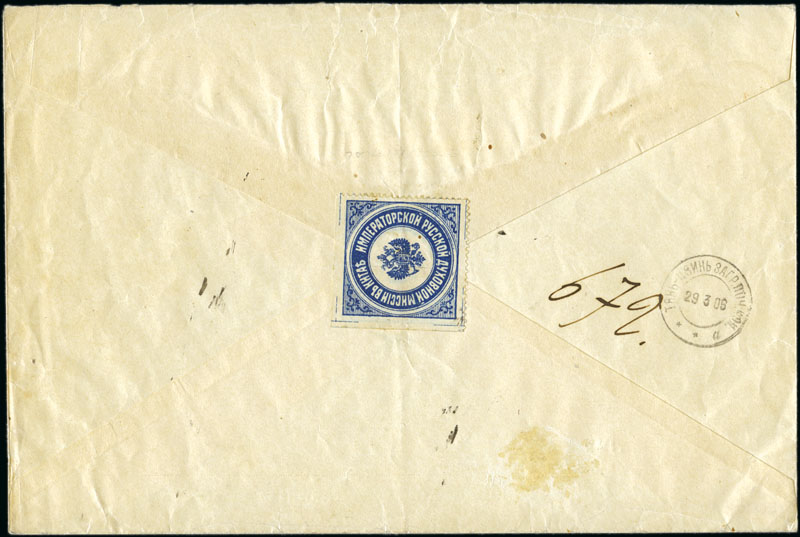
\includegraphics[width=.95\textwidth]{../russian-post-offices-in-china/10037-1.jpg}
\caption{
10037	PEKING: 1906 Cover registered to Tientsin franked with ordinary 
Russian 7k tied by Peking 28.3.06 cds (T\&S type 6) paying the reg'n 
fee on the obverse and Imperial Eagle free-frank seal on the reverse 
reading "Imperial Russian Ecclesiastical Mission to China," reg'd label 
in Cyrillic on obverse, a rare free franking.
\euro 300.00
}  
\end{figure}

\begin{figure}[htbp]
\centering
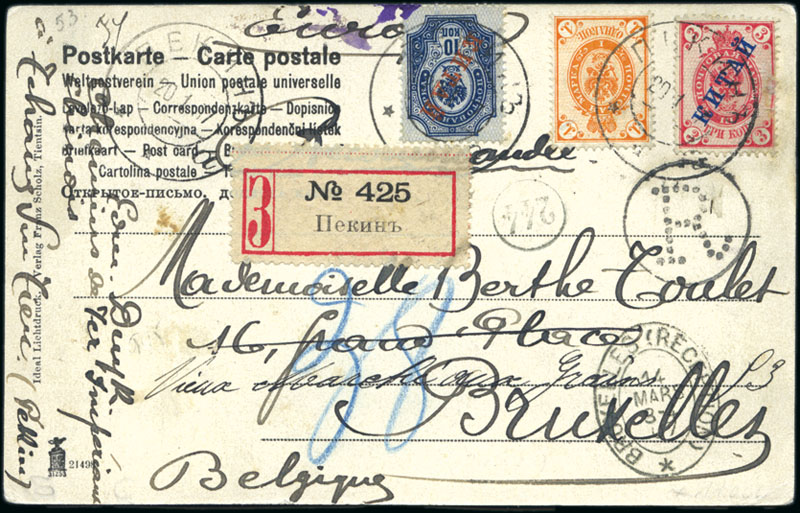
\includegraphics[width=.95\textwidth]{../russian-post-offices-in-china/10038.jpg}
\caption{
10038	PEKING: 1907 Postcard registered to Belgium with combination of 
ordinary Russian 1k and "KITAI" 3k and 10k, all tied by Peking 20.1.07 
cds (T\&S type 7A), sent by foreign national working on the Imperial Chinese 
Railway, with reg'd label in Cyrillic and encircled "dotted R," Brussels 
arrival, a scarce combination and cancellation
\euro 200.00
}  
\end{figure}

\begin{figure}[htbp]
\centering
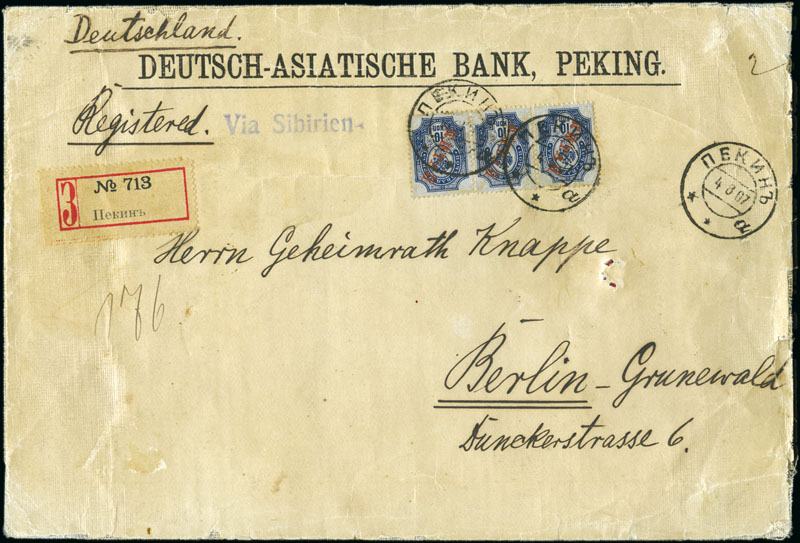
\includegraphics[width=.95\textwidth]{../russian-post-offices-in-china/10039.jpg}
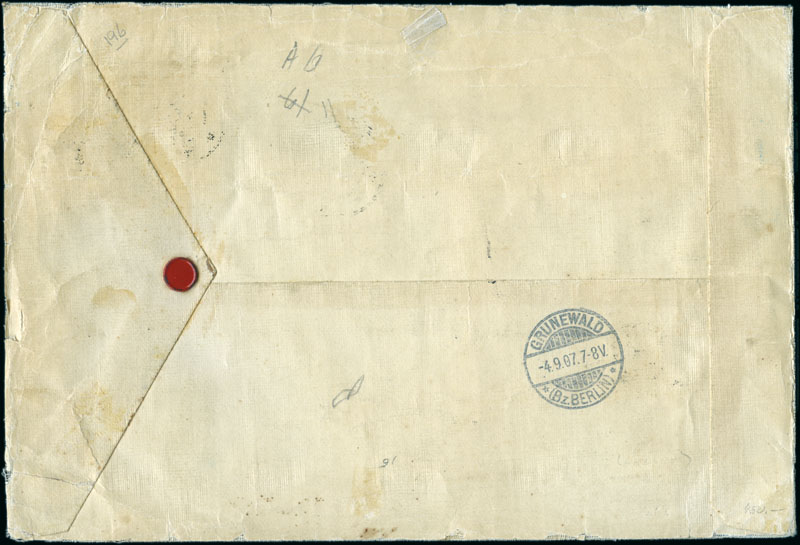
\includegraphics[width=.95\textwidth]{../russian-post-offices-in-china/10039-1.jpg}
\caption{
10039 PEKING: 1907 Cover registered to Germany with "KITAI" 10k in 
strip of three tied by scarce Peking 4.8.07 cds (T\&S type 7A), registered 
label adjacent, Berlin bs
\pound 200.00 
}  
\end{figure} 

\begin{figure}[htbp]
\centering
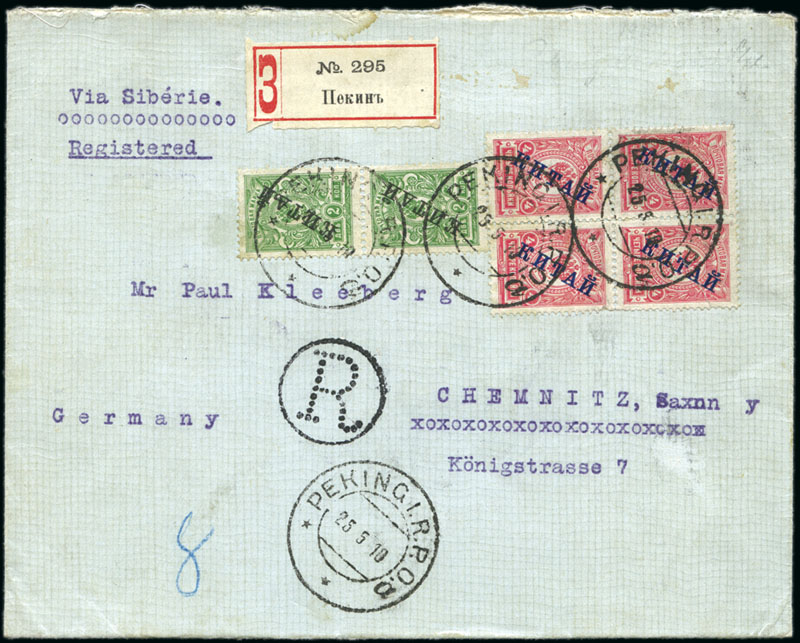
\includegraphics[width=.95\textwidth]{../russian-post-offices-in-china/10040.jpg}
\caption{
10040	PEKING: 1910 Cover registered from the Postmaster at Peking to Germany 
with "KITAI" 2k vert. pair and 4k block of four tied by Peking 25.5.10 cds 
(T\&S type 8, Gregorian calendar), with reg'd label in Cyrillic and encircled 
"dotted R" hs, St. Petersburg and Chemnitz bs.
The cancellation was introduced in 1910 by the Peking Postmaster for 
correspondence going abroad, but is rarely seen and was probably suppressed 
by the Imperial Russian Postal Administration. The contents of this cover 
(in German) give a brief history of the Russian P.O. at Peking, detailing
the stamps on sale, and providing examples of the cancels in use at his office. 
He explains that the type 8 cancel was his initiative for correspondence 
going abroad, and provides the only known strike of another of his 
innovations: the double oval "Doplatit" (To Pay) hs of Peking.
A truly fascinating piece of history of the Russian Post Office in Peking.
\euro 1,500.00. 
}  
\end{figure}  

\begin{figure}[htbp]
\centering
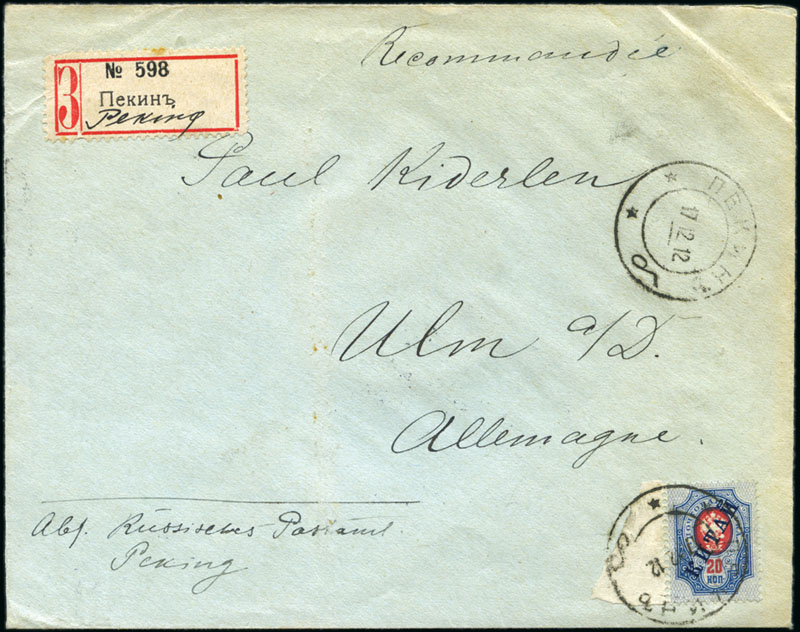
\includegraphics[width=.95\textwidth]{../russian-post-offices-in-china/10041.jpg}
\caption{
10041 PEKING: 1912 Cover registered to Germany with "KITAI" 20k tied by 
Peking 17.12.12 cds (T\&S type 7B), with registered label in Cyrillic 
adjacent with ms notation in English to comply with UPU regulations, 
reverse with wax seal showing Imperial Eagle and "Peking Post Office 
Abroad," Ulm Station bs, opened on 3 sides, a rare and unusual cover 
with this reg'n label and wax seal.
\euro 500.00. 
}  
\end{figure}   















    